\documentclass[useAMS,usenatbib,usegraphicx]{mn2e}

\def\l{{\ell}}
\def\lm{{\l m}}
\def\summ{\sum_{m=-\ell}^{\ell}}
\def\suml{\sum_{\ell=0}^{\infty}}
\def\alm{a_{\lm}}
\def\ylm{Y_{\lm}}
\def\cl{C_{\l}}



\title[Zonal Modes of CMB Temperature Maps]{Zonal Modes of Cosmic Microwave Background Temperature Maps}
\author[Short \& Coles]{Jo Short\thanks{Email: ShortJ1@cardiff.ac.uk (JS); Peter.Coles@astro.cf.ac.uk (PC)}
 and Peter Coles\\
 School of Physics and Astronomy, Cardiff University,
  Queens Buildings, 5 The Parade, Cardiff, CF24 3AA, United Kingdom.}

\begin{document}

\maketitle

\begin{abstract}
All-sky maps of the cosmic microwave background temperature
fluctuations are usually represented by a spherical harmonic
decomposition involving modes labelled by their degree $l$ and order
$m$ (where $-l\leq m \leq +l$). The {\em zonal modes} (i.e those
with $m=0$) are of particular interest because they vary only with
galactic latitude; any anomalous behaviour in them might therefore
be an indication of erroneous foreground substraction. We perform a
simple statistical analysis of the modes with low $l$ for sky maps
derived via different cleaning procedures from the Wilkinson
Microwave Anisotropy Probe (WMAP) and show that the zonal modes
provide a useful diagnostic of possible systematics.
\end{abstract}

\begin{keywords}
cosmology: cosmic microwave background --- cosmology: observations
--- methods: data analysis
\end{keywords}


\section{Introduction}

Observations of the temperature anisotropies of the cosmic microwave
background, particularly those from the Wilkinson Microwave
Anisotropy Probe (WMAP) \citep{b1,b3}, form the foundations of 
the remarkably successful ``concordance'' cosmological model
\citep{Colesb}.  An essential ingredient of this model is the
assumption that the primordial density fluctuations that seeded the
formation of galaxies and large-scale structure were statistically
homogeneous and Gaussian. Versions of the inflation scenario based
on the idea of a single slow-rolling scalar field predict levels of
non-Gaussianity too small to be observed. On the other hand,
multi-field inflation models and models with a non-standard kinetic
term for the inflaton may yield larger non-Gaussian effects which
could in principle be detected in current or next-generation
observations
\citep{BMR2002,BU2002,lyth2003,dvali2004,ACMZ2004,AST2004,BKMR2004,Chen2007,BB2007,KMVW2007}.
Analysis of currently available WMAP data provide strong limits on
the level of non-Gaussianity
\citep{Komatsu2003,Spergel2007,Creminelli2007,hikage}. On the other
hand, \citet{YW2007} recently reported a detection of primordial
non-Gaussianity at greater than 99.5\% significance. Further
detailed analyses of non-Gaussianity are clearly necessary in order
to reconcile and understand the various constraints and claimed
detections.

The greatest barrier to the detection of non-Gaussianity or other
departures from the framework of the concordance cosmological model
is the presence of residual foreground contamination or other
systematic errors. Since our own Galaxy emits at microwave
frequencies the emission from local foregrounds must be carefully
cleaned before a map can be obtained that is suitable for analysis.
One way of avoiding this problem is to cut out regions near the
Galactic plane where contamination is particularly severe but this
throws away the advantage of having full coverage. It is therefore
important to produce maps that are as clean as possible over the
whole sky for many purposes. However, such cleaning is inevitably
approximate and biases are bound to occur \citep{b6,nvn,cnc3}.
Circumstantial evidence exists that may be interpreted as residual
Galactic foregrounds in the WMAP data \citep{cnc2,ch07} but in the
absence of a more complete characterization of the galactic emission
the situation remains unclear.

In this {\em Letter} we propose and test a simple diagnostic test
that offers the possibility of identifying foreground-related biases
and systematics in all-sky maps of the CMB.

\section{Zonal Modes of CMB Maps}

The statistical variation of the CMB temperature $T(\theta,\varphi)$
over the celestial sphere can be conveniently decomposed into
spherical harmomic modes:
\begin{equation}
T(\theta,\varphi)=\suml \summ \alm \ylm (\theta,\varphi),
\end{equation}
where the $\ylm(\theta,\varphi) $ are spherical harmonic functions,
defined in terms of the Legendre polynomials $P_\lm$ using
\begin{equation}
\ylm(\theta,\varphi)=(-1)^m
\sqrt{\frac{(2\l+1)(\l-m)!}{4\pi(\l+m)!}}P_\lm(\cos\theta)e^{i m
\varphi},
\end{equation}
and the $\alm$ are complex coefficients which can be expressed with
$\alm=|\alm| \exp(i \Phi_\lm)$ and $\Phi_\lm$ are the phases
\citep{coles,cnc1,cnc2,cnc3,sc}; we have adopted the Condon-Shortly
phase definition in the spherical harmonic decomposition.

The spherical harmonics  $\ylm$ can be visualized by considering
their {\em nodal lines}, i.e. the set of points on the sphere where
they vanish. Nodal lines are circles, which are either in the
latitude or longitude direction with respect to the coordinate
system being used; in the case of CMB maps this is usually the
galactic coordinate system. The number of nodal lines of each type
is determined by the number of zeros of  $\ylm$ in the latitudinal
and longitudinal directions independently. The associated Legendre
functions $P_\lm$ possess $\l-|m|$ zeros in the latitude direction,
whereas the trigonometric $\sin$ and $\cos$ functions possess $2|m|$
zeros in the longitude direction. Two specific orders $m$ are of
particular interest at a given $l$ in the context of this work:
these denote the {\em zonal} modes, with $m=0$, and the {\em
sectoral} modes, with $m=\l$. In the former case there are no
zero-crossings in the longitude direction, so contours of equal
temperature run parallel to latitude lines; in the latter the
contours run parallel to longitude lines. Examples are shown in
Figure 1. In the intermediate cases with $0<m<\l$ there are
zero-crossings in both directions, giving rise to a patchwork
appearance; these are usually called {\em tesseral} modes.
\begin{figure}
  \centering
  \includegraphics[width = 84mm]{mapl10m0.ps}
  \includegraphics[width = 84mm]{mapl10m10.ps}
  \caption{Illustrative examples of zonal and sectoral modes for $\l=10$; the first example is the
  zonal mode with $m=0$ and the second is the sectoral mode with $m=10$.}
  \label{fig1}
\end{figure}


Statistically isotropic Gaussian random CMB temperature fluctuations
on a sphere, of the type that result from the simplest versions of
the inflationary paradigm, possess spherical harmonic coefficients
$\alm$ whose real and imaginary parts are mutually independent and
both Gaussian, or equivalently, the amplitudes $|\alm|$ are Rayleigh
distributed with random phases \citep{be,coles}. The statistical
properties of the fluctuations are then completely specified by the
angular power spectrum $\cl$,
\begin{equation}
\langle  a^{}_{\l^{ } m^{ }} a^{*}_{\l^{'} m^{'}} \rangle = \cl \;
\delta_{\l^{ } \l^{'}} \delta_{m^{} m^{'}}.
\end{equation}
Since $T$ is always real, the complex vectors of the $\alm$ on the
Argand plane for $m<0$ are mirror images of those with $m>0$ with
respect to $x$ axis for even $m$, and with respect to $y$ axis for
odd $m$. Writing \begin{equation} \alm = x_\lm + i y_\lm,
\end{equation}
we note that the variances of the real and imaginary parts of $\alm$
for $m>0$ are equal
\begin{equation}
\sigma^2(x_{\lm})=\sigma^2(y_{\lm})\equiv
\sigma^2_{\l}=\frac{1}{2}\cl,
\end{equation}
which depends only on $\l$. The distributions of $x_{\lm}$ and
$y_{\lm}$ are independent Gaussians with these variances and zero
mean. The amplitudes for these modes therefore have a Rayleigh
distribution \citep{be,sc}. For $m=0$, the imaginary part of $\alm$
must be zero, so this mode always has zero phase $\Phi_{\lm}$ and
the imaginary parts $y_{\lm}$ are consequently zero. This is because
the phase relates to the variation around the polar axis only.
However, the distribution $x_{\lm}$ for $m=0$ should be equal to
that of the other real parts at a given $\l$, namely a Gaussian with
zero mean and stated variance.



\section{Statistical Analysis}

Statistical analysis of the spherical harmonics of CMB maps usually
involves using all modes in an equivalent manner. However, since the
zonal modes in particular have such a special relationship to the
galactic coordinate system, it is worth looking at their properties
independently to see whether they hold any clues to possible
residual contamination aligned with the Galactic plane.

In order to construct a test which involved the smallest possible
number of assumptions - and in particular avoided the need to make
estimates of the power-spectrum $\cl$ along the way - we focussed on
the modes with maximum or minimum amplitude at a given $\l$. If all
modes are statistically equivalent (up to the differences noted in
the previous section) then the different orders $m$ at a given $\l$
are equally likely to furnish the maximum (or minimum) amplitude
$|\alm|$. A preference for modes with $m=0$ to display the maximum
(or minimum) amplitude might plausibly be interpreted as evidence
that the zonal modes are either contaminated with residual
foreground or that foregrounds have been excessively subtracted
\citep{cnc3,ch07,nvn}.

The maps considered here are the 1 \citep{b1}, 3 \citep{b2}, and 5
year \citep{b3} Internal Linear Combination (ILC) maps from the WMAP
team, the 1 and 3 year maps from \cite{b4} and the harmonic ILC map
by \cite{b5}. Because the variance of $\alm$ depends on $\l$ and the
variance of $\alm$ is in any case different for $m=0$ for $m\neq 0$
at a fixed $l$, it is not possible to obtain an analytical formula
for the expected number of times that the extremal amplitude occurs
at $m=0$ in general. However, we can finesse this difficulty by
instead comparing the actual maps with simulations constructed
according to the Gaussian assumption described in Section 2. We use
a set of simulations performed by \cite{b6}, which include ''raw''
sky maps and maps recovered using the the ILC methodology to remove
simulated foregrounds. These are particularly useful as they allow
us to assess whether any anomalies found are above the level known
to be introduced by the cleaning process.
\begin{table}
  \begin{tabular}{|c|c|c||c|c|c|}
    \hline \hline
    Map & max $\l$ & $m_{\rm min}=0$ & $m_{\rm max}=0$  & $m_{\rm min}=\l$ & $m_{\rm max}=\l$ \\ \hline
    ILC1     & 10 & 6    & 3  &  3    &  4    \\
    ILC3     & 10 & 7    & 2  &  2    &  4    \\
    ILC5     & 10 & 7    & 2  &  2    &  4    \\
    Teg1     & 10 & 6    & 2  &  3    &  4    \\
    Teg3     & 10 & 8    & 2  &  2    &  4    \\
    HILC     & 10 & 8    & 2  &  1    &  5    \\ \hline
    ILC1     & 20 & 9    & 3  &  3    &  6    \\
    ILC3     & 20 & 9    & 2  &  2    &  5    \\
    ILC5     & 20 & 8    & 2  &  2    &  4    \\
    Teg1     & 20 & 8    & 3  &  3    &  5    \\
    Teg3     & 20 & 11   & 2  &  2    &  5    \\
    HILC     & 20 & 10   & 2  &  1    &  6    \\ \hline
    \hline
  \end{tabular}
  \caption{Number of occurrences of $m_{\rm ext}=0$ or $\l$ in selected CMB maps.}
  \label{TABnum}
\end{table}
We identified the value of $m$ associated with the largest (or
smallest) amplitude for a given $\l$ for the ranges $[0,10]$ and
$[0,20]$; the number of times where this was the zonal mode is given
in Table \ref{TABnum}. We have restricted our analysis to low $\l$ modes partly to
keep the computational cost of the simulations down and partly
because the high $\l$ modes are known not to be clean anyway. We have also given results for the sectoral
modes for comparison, but there are no significant anomalies
associated with them and we shall not discuss them further in this
paper.  As can be seen in Table \ref{TABsig}, for the case of zonal maxima but the
zonal minima do show a significant result for zonal modes with low
amplitudes in the \cite{b4} 3 yr and the \cite{b5} HILC maps for
$\l<10$. It is also interesting to note is that the Tegmark et al. 3
yr gives a higher significance level than the Tegmark et al. 1 yr
map, as does the WMAP ILC 5 yr map compared to the corresponding 1
yr map.
\begin{table}
  \begin{tabular}{|c|c|c||c|c|c|}
    \hline \hline
    Map & max $\l$ & $m_{\rm min}=0$ & $m_{\rm max}=0$ & $m_{\rm min}=\l$ & $m_{\rm max}=\l$ \\ \hline
    ILC1&   10&      50.42 &    1.75  &             28.45 &             60.88\\
    ILC3&   10&       83.48 &   69.28 &              0.00 &             60.88\\
    ILC5&   10&       83.48 &   69.28 &              0.00 &             60.88\\
    Teg1&   10&  50.42 &    69.28 &             28.45 &             60.88\\
    Teg3&   10&       96.30 &   69.28 &              0.00 &             60.88\\
    HILC&   10&       96.30 &   69.28 &             49.11 &             89.88\\ \hline
    ILC1&   20&  76.02 &    48.99 &              0.00 &             85.68\\
    ILC3&   20&  76.02 &    87.34 &              6.41 &             60.18\\
    ILC5&   20&       48.17 &   87.34 &              6.41 &             14.13\\
    Teg1&   20&  48.17 &    48.99 &              0.00 &             60.18\\
    Teg3&   20&  96.88 &        87.34 &              6.41 &             60.18\\
    HILC&   20&  90.08 &    87.34 &             68.62 &                 85.68\\ \hline
    \hline
  \end{tabular}
  \caption{Significance of occurrences of $m_{\rm ext} = 0$ or $\l$ in selected CMB maps.}
  \label{TABsig}
\end{table}

We performed a further investigation in order to locate the source
of the apparent deficit in the zonal modes. The variance of the
distribution of the real values of the $\alm$ for $m=0$ was compared
between the ILC 5 yr and the Tegmark et al. 3 yr maps and the
simulations. We found evidence that  the variance of the $m = 0$
reals in the ILC 5 yr and the Tegmark et al. 3 yr maps is smaller
than in the simulations (94\% and 95\% respectively), which is
consistent with the previously reported low variance in the ILC map
by \cite{b7}. This leads to the further question of whether the
zonal mode  amplitudes are entirely responsible for this low
variance. Table \ref{TABvar} shows that by removing the $m = 0$
 amplitudes the number of simulated maps with a variance
greater than the test map falls dramatically.

\begin{table}
\begin{center}
  \begin{tabular}{|c|c|c|c|}
    \hline \hline
    Map & $m = 0$ & $\forall m$ & $m\ne 0$    \\ \hline
    ILC5  &  97.14  & 93.18 &    68.99             \\
    Teg3  &  97.57  & 93.76 &    69.23            \\  \hline
    \hline
  \end{tabular}
  \caption{Percentage of simulations with $x_{\lm}$, for given $m$, which have variance greater than the specified map}
  \label{TABvar}
\end{center}
\end{table}

\begin{figure}
  \centering
  \includegraphics[width = 84mm]{wmap5_map.ps}
  \caption{Reconstructed CMB map for WMAP ILC 5 yr map using only the $m=0$ modes for $\l = [0,20]$}
  \label{fig2}
\end{figure}
It is interesting to reconstruct what the CMB sky would look like if
it only contained the zonal modes; the result in Figure \ref{fig2}
shows that the deepest minima are just above and below the Galactic
plane. We tested whether these minima are of abnormally low
amplitude compared to the simulated maps. Because the resolution of the
maps is quite low, we restricted our analysis to the parts of the
map that are well-sampled (i.e. we neglected the Galactic pole
areas). Monte Carlo simulations were run to estimate the probability
of a maximum or minimum as seen in the map. The resulting
significance levels are shown in Table \ref{TABcol}.
\begin{table}
\begin{center}
  \begin{tabular}{|c|c|c|}
    \hline \hline
    Map &  minimum &  maximum \\ \hline
    ILC1     &  46.00  &   76.26    \\
    ILC3     &  64.18  &   97.70  \\
    ILC5     &  62.48  &   98.04    \\
    Teg1     &  55.76  &   90.00         \\
    Teg3     &  90.42  &   97.26      \\
    HILC     &  70.70  &   95.88      \\ \hline
    \hline
  \end{tabular}
  \caption{Significance levels of the maxima and minima in zonal maps, as derived from Monte Carlo simulations.}
  \label{TABcol}
\end{center}
\end{table}
The trend revealed in this table again seems to be that some form of
anomaly associated with the zonal modes is present and that it
becomes increasingly significant as the maps supposedly improve!

\section{Discussion}
We have presented a simple statistical analysis based on properties
of the zonal modes of cosmic microwave background maps, i.e. those
aligned parallel to the Galactic plane. An application of the test
to various cleaned CMB maps gives interesting results. At the 95 per
cent level, no significant anomalies appear in the WMAP ILC maps
\citep{b1,b2,b3} but there seems to be a significant tendency in
some other maps \citep{b4,b5} to have zonal modes with
systematically lower amplitudes than would be expected in the
concordance model. Intriguingly, the maps that provide the most
significant departures from the behaviour expected under the null
hypothesis are those based on later issues of the WMAP data. This
could be because there is a systematic problem that becomes more
obvious when the noise levels are lower.

It must be noted that the significance levels we quote of around 96
to 97 percent are not overwhelming so the results we have obtained
are indicative rather than decisive. This is not surprising, given
the relatively small number of modes we used. However, we repeated
the analysis for a coordinate system aligned with the Ecliptic,
rather than Galactic plane and found no significant results at all.
This lends further credence to our interpretation of the outcome of
our analysis in terms of an effect related to over-subtraction of
Galactic emission \citep{cnc3,nvn}. A more definitive result will
have to wait until more detailed foreground subtraction can be
attempted, such as will be the case with the {\em Planck} satellite.



\section*{Acknowledgements}
Jo Short receives support from a Science \& Technology
Facilities Council (STFC) doctoral training grant. We would like to
thank Pavel Naselsky for interesting discussions. We gratefully
acknowledge the use of the HEALPIX package \citep{heal}.



\begin{thebibliography}{99}
\bibitem[\protect\citeauthoryear{Alishahiha et al.}{2004}]{AST2004}
  Alishahiha M., Silverstein  E., Tong D., 2004,
  Phys. Rev. D., 70, 123505
  \bibitem[\protect\citeauthoryear{Arkami-Hamed et al.}{2004}]{ACMZ2004}
  Arkani-Hamed N., Creminelli P., Mukohyama S., Zaldarriaga M., 2004,
  JCAP, 4, 1
\bibitem[\protect\citeauthoryear{Bartolo et al.}{2002}]{BMR2002}
  Bartolo N., Matarrese S., Riotto A., 2002, Phys. Rev. D., 65, 103505
  \bibitem[\protect\citeauthoryear{Bartolo et al.}{2004}]{BKMR2004}
  Bartolo N., Komatsu E., Matarrese S., Riotto A., 2004, Phys. Rept., 402, 103
  \bibitem[\protect\citeauthoryear{Battefeld \& Battefeld}{2007}]{BB2007}
  Battefeld D., Battefeld T., 2007, JCAP, 5, 1
\bibitem[\protect\citeauthoryear{Bennett et al.}{2003}]{b1} Bennett C. L.  et al., 2003, ApJS, 148,
1
\bibitem[\protect\citeauthoryear{Bernardeau \& Uzan}{2002}]{BU2002}
  Bernardeau F., Uzan J.-P., 2002,  Phys. Rev. D., 66, 103506
\bibitem[\protect\citeauthoryear{Bond \& Efstathiou}{1987}]{be}
Bond J. R., Efstathiou G., 1987, MNRAS, 226, 655
\bibitem[\protect\citeauthoryear{Chen et al.}{2007}]{Chen2007}
  Chen X., Easther R., Lim E. A., 2007, JCAP, 6, 23
\bibitem[\protect\citeauthoryear{Chiang, Naselsky \& Coles}{2004}]{cnc1}
Chiang L.-Y., Naselsky P. D., Coles P., 2004, ApJ, 602, L1
\bibitem[\protect\citeauthoryear{Chiang, Naselsky \& Coles}{2007}]{cnc2}
Chiang L.-Y., Naselsky P. D., Coles P., 2007, ApJ, 664,8
\bibitem[\protect\citeauthoryear{Chiang, Naselsky \& Coles}{2009}]{cnc3}
Chiang L.-Y., Naselsky P. D., Coles P., 2009, ApJ, 694, 339
\bibitem[\protect\citeauthoryear{Chiang et al.}{2007}]{ch07}
Chiang L.-Y., Coles P., Naselsky P. D., Olesen P., 2007, JCAP, 1, 21
\bibitem[\protect\citeauthoryear{Coles} {2005}]{Colesb} Coles P., 2005, Nat, 433, 248
\bibitem[\protect\citeauthoryear{Coles et al.}{2004}]{coles}
 Coles P., Dineen P., Earl J., Wright D., 2004, MNRAS, 350, 989
\bibitem[\protect\citeauthoryear{Creminelli et al.}{2007}]{Creminelli2007}
  Creminelli P., Senatore L., Zaldarriaga M., \&
  Tegmark M., 2006, JCAP, 03, 005
 \bibitem[\protect\citeauthoryear{Dvali et al.}{2004}]{dvali2004}
  Dvali G., Gruzinov A., Zaldarriaga M., 2004,
  Phys. Rev. D., 69, 083505
\bibitem[\protect\citeauthoryear{Eriksen et al.}{2005}]{b6} Eriksen H. K.  et al., 2005, astro-ph/0508196
\bibitem[\protect\citeauthoryear{G\'{o}rski et al.}{2005}]{heal} G\'{o}rski K. M., Hivon E., Banday A. J., Wandelt B. D.,
Hansen F. K., Reinecke E. M., Bartelmann M., 2005, ApJ, 622, 759
\bibitem[\protect\citeauthoryear{Hikage et al.}{2008}]{hikage}
Hikage C., Matsubara T., Coles P., Liguori M., Hansen H. K.,
Matarrese S., 2008, MNRAS, 389, 1439
\bibitem[\protect\citeauthoryear{Hinshaw et al.}{2009}]{b3} Hinshaw G.  et al., 2009, ApJS, 180, 225
\bibitem[\protect\citeauthoryear{Jarosik et al.}{2007}]{b2} Jarosik N.  et al., 2007, ApJS, 170, 263
\bibitem[\protect\citeauthoryear{Kim et al.}{2008}]{b5} Kim J. et
al., 2008, Phys. Rev. D, 77, 103002
\bibitem[\protect\citeauthoryear{Komatsu et al.}{2003}]{Komatsu2003}
  Komatsu E. et al., 2003, ApJS, 148, 119
\bibitem[\protect\citeauthoryear{Koyama et al.}{2007}]{KMVW2007}
  Koyama K., Mizuno S., Vernizzi F., Wands D., 2007, JCAP, 11, 24
\bibitem[\protect\citeauthoryear{Lyth et al.}{2003}]{lyth2003}
  Lyth D. H., Ungarelli C., Wands D., 2003,
  Phys. Rev. D., 67, 23503
\bibitem[\protect\citeauthoryear{Monteserin et al.}{2007}]{b7} Monteserin C.  et al., 2007, MNRAS, 387, 209
\bibitem[\protect\citeauthoryear{Naselsky, Verkhodanov \&
Nielsen}{2008}]{nvn} Naselsky P. D., Verkhodanov O. V., Nielsen M.
T. B., 2008, AstBu,  63, 216
\bibitem[\protect\citeauthoryear{Spergel et al.}{2007}]{Spergel2007}
  Spergel  D.N. et al., 2007, ApJS, 170, 377
\bibitem[\protect\citeauthoryear{Stannard \& Coles}{2006}]{sc}
Stannard A., Coles P., 2005, MNRAS, 364, 929
\bibitem[\protect\citeauthoryear{Tegmark et al.}{2003}]{b4} Tegmark M. et al., 2003, Phys. Rev. D, 68, 123523
\bibitem[\protect\citeauthoryear{Yadav \& Wandelt}{2007}]{YW2007}
  Yadav A. P. S., Wandelt B. D., 2007, Phys. Rev. Lett., 100, 181301
\end{thebibliography}



\end{document}
